\documentclass[../main.tex]{subfiles}

\begin{document}
	\begin{ese}[7.1]
		Dare i valori di spin e parità attesi secondo il modello a shell per gli stati fondamentali di: $ ^{7}\chem{Li},\ ^{11}\chem{B},\ ^{15}\chem{C},\ ^{17}\chem{F},\ ^{31}\chem{P},\ ^{141}\chem{Pr} $
	\end{ese}
	\begin{svol}
		In generale, nello studio di spin e parità di nuclei conseguente al modello a shell ci sono tre casistiche possibili:
		\begin{enumerate}
			\item[Pari-pari] Nel caso di atomi pari-pari, ossia con un numero pari sia di protoni che di neutroni tutti questi sono accoppiati e lo spin totale è zero e la parità è positiva.
			\item[Pari-dispari] Nel caso in cui un tipo di nucleone non sia pari uno di questi rimane disaccoppiato e lo spin del nucleo è uguale al valore di momento angolare totale del nucleone non accoppiato. La parità è uguale a $ (-1)^{l} $ dove $ l $ è il numero quantico associato al valore di momento angolare orbitale del nucleone più esterno (quello disaccoppiato).
			\item[Dispari-dispari] Nel caso in cui ci fossero sia un protone che un neutrone disaccoppiati, con numeri quantici associati al momento angolare totale uguali a $ j_{1} $ e $ j_{2} $ rispettivamente, lo spin totale nucleare è la somma di questi. Lo spin nucleare può quindi prendere tutti valori compresi nel range:
			\begin{gather*}
			\left|j_{1}-j_{2}\right|\leq j_{N}\leq j_{1}+j_{2}
			\end{gather*}
			La parità del nucleo è data da $ (-1)^{(l_{1}+l_{2})} $ dove $ l_{1} $ ed $ l_{2} $ sono i numeri quantici associati al momento angolare orbitale del (rispettivamente) protone e neutrone più esterno.
		\end{enumerate}
		Per tutti i seguenti casi si farà uso della tabella presentata a lezione degli orbitali nel modello a shell e della tavola periodica degli elementi.
		
		Il $ ^{7}\chem{Li} $ ha tre protoni e quattro neutroni. Si è quindi nel caso 2. Il protone più esterno è nella shell $ 1p_{\frac{3}{2}} $ dunque lo spin totale del nucleo sarà $ \frac{3}{2} $. Il numero quantico associato alla shell $ p $ è $ l_{p}=1 $ dunque la parità è negativa.
		
		Il $ ^{11}\chem{B} $ ha cinque protoni e sei neutroni. Si è ancora nel caso 2. Il protone più esterno è nella shell $ 1p_{\frac{3}{2}} $ dunque lo spin totale del nucleo sarà $ \frac{3}{2} $. La parità è ancora negativa

		Il $ ^{15}\chem{C} $ ha sei protoni e nove neutroni. Si è ancora nel caso due. Il neutrone più esterno è nella shell $ 1d_{\frac{5}{2}} $ dunque lo spin totale sarà $ \frac{5}{2} $. Il numero quantico associato alla shell $ d $ è $ l_{d}=2 $ quindi la parità è positiva. 
		
		Il $ ^{17}\chem{F} $ ha nove protoni e otto neutroni. Si è ancora nel caso 2. Il protone più esterno è nella shell $ 1d_{\frac{5}{2}} $ dunque lo spin totale sarà $ \frac{5}{2} $. La parità è ancora positiva.
		
		Il $ ^{31}\chem{P} $ ha 15 protoni e 16 neutroni. Si è ancora nel caso 2. Il protone più esterno è nella shell $ 2s_{\frac{1}{2}} $ dunque lo spin totale sarà $ \frac{1}{2} $. Il numero quantico associato alla shell $ s $ è $ l_{s}=0 $ dunque la parità è positiva.
		
		Il $ ^{141}\chem{Pr} $ ha 59 protoni e 82 neutroni. Si è ancora nel caso 2. Il protone più esterno è nella shell $ 1g_{\frac{7}{2}} $ dunque lo spin totale sarà $ \frac{7}{2} $. Il numero quantico associato alla shell $ g $ è $ l_{g}=4 $ dunque la parità è positiva.
		
		Tutti i risultati ottenuti combaciano con quelli sperimentali ad eccezione del terzo. Il carbonio $ 15 $ in fatti, si misura avere spin $ 1/2 $. Questo risultato non è previsto dalla teoria e necessita ulteriori approfondimenti.
	\end{svol}
	\newpage
	\begin{ese}[7.5]
		Nel modello a shell, le proprietà dello stato fondamentale dei nuclei dispari-dispari dipende dall'interazione di protone e neutrone, ovvero da $ \vec{J}=\vec{j}_{p}+\vec{j}_{n} $. Considerando i nuclei $$ ^{16}\chem{N}(2^{-}),\ ^{12}\chem{B}(1^{+}),\ ^{34}\chem{P}(1^{+}),\ ^{28}\chem{Al}(3^{+}) $$ da un semplice diagramma vettoriale indicare la posizione relativa di $ \vec{j}_{p} $ e $ \vec{j}_{n} $. Sostituire $ \vec{j}_{p}=\vec{l}_{p}+\vec{s}_{p} $ e derivare una regola empirca per l'orientazione relativa degli spin di $ p $ ed $ n $. Usare tale regola per predire $ J^{P} $ dello stato fondamentale di $ ^{26}\chem{Na} $ e $ ^{28}\chem{Na} $.
	\end{ese}
	\begin{svol}
		Il $ ^{16}\chem{N}(2^{-}) $ ha sette protoni e nove neutroni. Il protone più esterno occupa la shell $ 1p_{\frac{1}{2}} $ e il neutrone più esterno occupa la shell $ 1d_{\frac{5}{2}} $. Perciò i momenti angolari totali sono rivolti in direzione opposta. Inoltre per il protone, per permettere che il momento angolare totale sia $ \frac{1}{2} $ è necessario che il momento angolare di spin e quello orbitale siano antiparalleli. Per il neutrone questi sono invece paralleli. Il grafico corrispondente a questa disposizione è presente in figura \ref{fig:16N}.
		\begin{figure}[h]
			\centering
			\begin{tikzpicture}
				\draw[thick,->] (0,-1) -- (0,1) node[anchor=north east] {$p$ orbit}; 
				\node[] at (1,0)  {+};
				\draw[thick,->] (2,1/2) -- (2,-1/2) node[anchor=north east] {$ p $ spin};
				\node[] at (3,0) {+};
				\draw[thick,->] (4,2) -- (4,-2) node[anchor=north east] {$ n $ orbit};
				\node[] at (5,0){+};
				\draw[thick,->] (6,1/2) -- (6,-1/2) node[anchor=north east] {$ n $ spin};
			\end{tikzpicture}
			\caption{Posizinamento dei momenti angolari orbitali e di spin nel nucleo di $ ^{16}\chem{N} $}\label{fig:16N}
		\end{figure}

	
		
		Il $ ^{12}\chem{B}(1^{+}) $ ha cinque protoni e sette neutroni. Il protone più esterno occupa la shell $ 1p_{\frac{3}{2}} $ e il neutrone più esterno occupa la shell $ 1p_{\frac{1}{2}} $. Perciò i momenti angolari totali sono rivolti in direzione opposta. Inoltre per il protone, per permettere che il momento angolare totale sia $ \frac{3}{2} $ è necessario che il momento angolare di spin e quello orbitale siano paralleli. Per il neutrone questi sono invece antiparalleli. Il grafico corrispondente a questa disposizione è presente in figura \ref{fig:12B}.
		\begin{figure}[h]
			\centering
			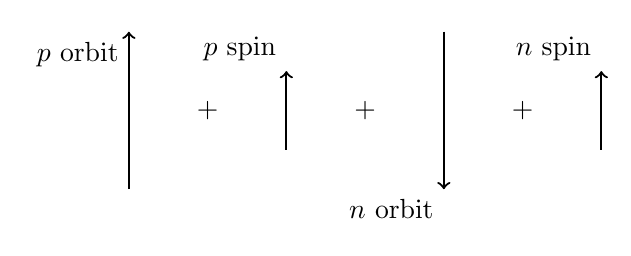
\begin{tikzpicture}
			\draw[thick,->] (0,-1) -- (0,1) node[anchor=north east] {$p$ orbit}; 
			\node[] at (1,0)  {+};
			\draw[thick,->] (2,-1/2) -- (2,1/2) node[anchor=south east] {$ p $ spin};
			\node[] at (3,0) {+};
			\draw[thick,->] (4,1) -- (4,-1) node[anchor=north east] {$ n $ orbit};
			\node[] at (5,0){+};
			\draw[thick,->] (6,-1/2) -- (6,1/2) node[anchor=south east] {$ n $ spin};
			\end{tikzpicture}
			\caption{Posizinamento dei momenti angolari orbitali e di spin nel nucleo di $ ^{12}\chem{B} $}\label{fig:12B}
		\end{figure}

	
	Il $ ^{34}\chem{P}(1^{+}) $ ha 15 protoni e 19 neutroni. Il protone più esterno occupa la shell $ 2s_{\frac{1}{2}} $ e il neutrone più esterno occupa la shell $ 1d_{\frac{3}{2}} $. Perciò i momenti angolari totali sono rivolti in direzione opposta. Il protone non ha momento angolare orbitale. Per il neutrone, per permettere un momento angolare totale di $ \frac{3}{2} $ è necessario che il momento angolare orbitale e quello di spin siano antiparalleli. Il grafico corrispondente a questa disposizione è presente in figura \ref{fig:34P}.
	
	\begin{figure}[h]
		\centering
		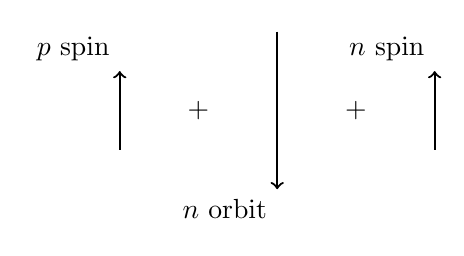
\begin{tikzpicture}
		
		\draw[thick,->] (2,-1/2) -- (2,1/2) node[anchor=south east] {$ p $ spin};
		\node[] at (3,0) {+};
		\draw[thick,->] (4,1) -- (4,-1) node[anchor=north east] {$ n $ orbit};
		\node[] at (5,0){+};
		\draw[thick,->] (6,-1/2) -- (6,1/2) node[anchor=south east] {$ n $ spin};
		\end{tikzpicture}
		\caption{Posizinamento dei momenti angolari orbitali e di spin nel nucleo di $ ^{34}\chem{P} $}\label{fig:34P}
	\end{figure}

	Il $ ^{28}\chem{Al}(3^{+}) $ ha 13 protoni e 15 neutroni. Il protone più esterno occupa la shell $ 1d_{\frac{5}{2}} $ e il neutrone più esterno occupa la shell $ 2s_{\frac{1}{2}} $. Perciò i momenti angolari totali sono rivolti in direzione parallela. Inoltre per il protone, per permettere che il momento angolare totale sia $ \frac{5}{2} $ è necessario che il momento angolare di spin e quello orbitale siano paralleli. Il neutrone non ha momento angolare orbitale. Il grafico corrispondente a questa disposizione è presente in figura \ref{fig:28Al}.
	
	\begin{figure}[h]
		\centering
		\begin{tikzpicture}
		
		\draw[thick,->] (0,-2) -- (0,2) node[anchor=north east] {$p$ orbit};
		\node[] at (1,0) {+};
		\draw[thick,->] (2,-1/2) -- (2,1/2) node[anchor=south east] {$ p $ spin};
		\node[] at (3,0) {+};
		\draw[thick,->] (4,-1/2) -- (4,1/2) node[anchor=south east] {$ n $ spin};
		\end{tikzpicture}
		\caption{Posizinamento dei momenti angolari orbitali e di spin nel nucleo di $ ^{28}\chem{Al} $}\label{fig:28Al}
	\end{figure}
	
	Da tutte le rappresentazioni grafiche di spin e momento angolare risulta che i momenti angolari di spin sono sempre paralleli l'uno all'altro. Si può usare questa regola euristica per dedurre i momenti angolari di totali dei nuclei richiesti.
	
	Il $ ^{26}\chem{Na} $ ha 11 protoni e 15 neutroni. Il protone più esterno occupa la shell $ 1d_{\frac{5}{2}} $ e il neutrone più esterno occupa la shell $ 2s_{\frac{1}{2}} $. Per il protone, per permettere che il momento angolare totale sia $ \frac{5}{2} $ è necessario che il momento angolare di spin e quello orbitale siano paralleli. Il neutrone non ha momento angolare orbitale. Dovendo gli spin essere paralleli l'uno all'altro si ha che tutti i momenti angolari si sommano, ottenendo così un momento angolare totale di $ 3 $. La situazione è completamente analoga a quella dell'alluminio 28, per cui ci si può aspettare una parità positiva.
	
	Il $ ^{28}\chem{Na} $ ha 11 protoni e 17 neutroni. Il protone più esterno occupa la shell $ 1d_{\frac{5}{2}} $ e il neutrone più esterno occupa la shell $ 1d_{\frac{3}{2}} $. Per il protone, per permettere che il momento angolare totale sia $ \frac{5}{2} $ è necessario che il momento angolare di spin e quello orbitale siano paralleli. Per il neutrone invece è necessario che questi siano antiparalleli. Dovendo gli spin essere paralleli l'uno all'altro si ha che i momenti angolari totali si sottraggono, ottenendo così un momento angolare totale di $ 1 $. La situazione è completamente analoga a quella dell'azoto 16, per cui ci si può aspettare una parità negativa.
	
	\end{svol}

\end{document}